\documentclass[11pt]{article}
\usepackage{fancyhdr} 
\pagestyle{fancy}
\fancyhf{}
\fancyheadoffset{0cm}
\renewcommand{\headrulewidth}{0pt} 
\renewcommand{\footrulewidth}{0pt}
\fancyhead[R]{{\color{gray!50}Page Number: \thepage { \small (out of 11 pages)}}}
\fancypagestyle{plain}{%
  \fancyhf{}%
  \fancyhead[R]{\thepage}%
}

\newcommand{\Ans}{Answer: }


\usepackage{graphicx}
\usepackage[margin=.5in]{geometry} 
\usepackage{amsmath,amsthm,amssymb}
%\usepackage{gensymb}
  \usepackage{hyperref}
  \usepackage{pdfpages} 
  %\usepackage[table]{xcolor}
  
 %\usepackage{xcolor} % Required for specifying colors by name
\definecolor{ocre}{RGB}{52,177,201} % Define the orange color used for highlighting throughout the book

% Font Settings
\usepackage{avant} % Use the Avantgarde font for headings
%\usepackage{times} % Use the Times font for headings
\usepackage{mathptmx} % Use the Adobe Times Roman as the default text font together with math symbols from the Sym­bol, Chancery and Com­puter Modern fonts

%\usepackage{microtype} % Slightly tweak font spacing for aesthetics
%\usepackage[utf8]{inputenc} % Required for including letters with accents
\usepackage[T1]{fontenc} % Use 8-bit encoding that has 256 glyphs
%\usepackage{soul}
\usepackage{undertilde}
%\usepackage{accents}
\newcommand{\StandardLM}{\by=\bX \bbeta +{\epsilonbf}}

\usepackage{xcolor}
\usepackage{xparse}
\definecolor{lightGray}{gray}{0.95}
\definecolor{lightGrayOne}{gray}{0.9}
\definecolor{lightBlueOne}{RGB}{204, 255, 255}
\definecolor{lightBlueTwo}{RGB}{204, 238, 255}
\definecolor{lightBlueThree}{RGB}{204, 204, 255}
\definecolor{AltBlue}{RGB}{119,14,161}
\definecolor{Orchid}{RGB}{186,85,211}

\definecolor{BGBlue}{RGB}{220,221,252}
\definecolor{BGBlueOne}{RGB}{204,229,255}

\definecolor{DarkGreenOne}{RGB}{34,139,34}

\definecolor{BGGreen}{RGB}{240,243,245}
\definecolor{lightGreenOne}{RGB}{179, 255, 179}
\definecolor{lightGreenTwo}{RGB}{198, 255, 179}
\definecolor{lightGreenThree}{RGB}{243, 255, 230}
\definecolor{AltGreen}{RGB}{193, 240, 240}

\definecolor{BOGreen}{RGB}{180,0,0}
\definecolor{BGGreenOne}{RGB}{220,250,220}

\definecolor{lightBrownOne}{RGB}{255, 221, 204}
\definecolor{lightBrownTwo}{RGB}{255, 229, 204}
\definecolor{lightBrownThree}{RGB}{242, 217, 230}


\definecolor{HLTGreen}{RGB}{230,244,215}
\definecolor{ExcBrown}{RGB}{153,0,0}
\definecolor{ExcBGBrown}{RGB}{255,204,204}
\definecolor{BGYellowOne}{RGB}{255,235,208}
\definecolor{BGPink}{RGB}{255,215,240}

\newcommand{\MakeVec}[1]{{\utilde{\bf #1}}}

\NewDocumentCommand{\MCOption}{O{1.75in} m}{
\TextInBoxTwo[BGPink]{ #1 } {\TextInBoxTwo[white]{.1 in }{ \quad}\HLT{#2}}
}

 \NewDocumentCommand{\ThreeChoices}{O{Do not Know}O{Not confident}O{Confident}}{
\MCOption{#1} \MCOption{#2} \MCOption{#3}
}
 
\NewDocumentCommand{\OneBlock}{ O{HLTGreen} m m }{\colorbox{#1}{\begin{minipage}{#2} $ #3$ \end{minipage}}}

\NewDocumentCommand{\HLT}{ O{HLTGreen} m }{\colorbox{#1}{#2}}
%\NewDocumentCommand{\HLTEQ}{ O{HLTGreen} m }{\colorbox{#1}{$#2$}}
\NewDocumentCommand{\HLTEQ}{ O{white} m }{\colorbox{#1}{$#2$}}

%\newcommand{\HLT}[1]{\colorbox{HLTGreen}{#1}}
\newcommand{\DEHLT}[1]{\colorbox{lightGrayOne}{\color{white} #1}}

\newcommand{\TextInBoxOne}[2]{  {\fcolorbox{white}{lightGrayOne}{\begin{minipage}{#1}  #2 \end{minipage}}}}


\NewDocumentCommand{\TextInBoxTwo}{ O{lightGrayOne} m m } {{\fcolorbox{white}{#1}{\begin{minipage}{#2} { #3} \end{minipage}}}}


\newcommand{\TextInBox}[2]{  {\fcolorbox{BGGreen}{BGGreen}{\begin{minipage}{#1}  #2 \end{minipage}}}}
\newcommand{\TextInBoxCol}[2]{
\fcolorbox{BGBlue}{BGBlue}{%
\begin{minipage}{#1}
 {\color{AltBlue} #2}
\end{minipage}}%
}

\NewDocumentCommand{\TxtBnd}{ O{lightBrownOne} m m } {{\fcolorbox{white}{#1}{\begin{minipage}{#2} { #3} \end{minipage}}}}


\newcommand{\BandInTopBox}[2]{
\fcolorbox{AltBlue}{AltBlue}{%
\begin{minipage}{#1}{ {\color{white}  #2 \hspace{.1in}} }
\end{minipage}}%
}


\newcommand{\TextInBoxThm}[2]{
\fcolorbox{AltBlue}{lightGray}{%
\begin{minipage}{#1}
 {\color{black} #2}
\end{minipage}}%
}

\newcommand{\TextInBoxThmOne}[2]{
\fcolorbox{BGBlue}{BGBlueOne}{%
\begin{minipage}{#1}
 {\color{AltBlue} #2}
\end{minipage}}%
}

\newcommand{\TextInBoxLem}[2]{
\fcolorbox{BGBlue}{lightGray}{%
\begin{minipage}{#1}
 {\color{black} #2}
\end{minipage}}%
}



\newcommand{\TextInBoxLemOne}[2]{
\vspace{.02 in}
\noindent
\fcolorbox{BGBlue}{BGBlue}{%
\begin{minipage}{#1}
 {\color{AltBlue} #2}
\end{minipage}}%
}



\newcommand{\DefBox}[1]{
%\vspace{.1 in}
\noindent
\TextInBoxLem{4.5 in }{
\BandInTopBox{4.4 in }{}
\TextInBoxLemOne{4.4 in }{
#1
}}}





\newcommand{\DefBoxOne}[2]{
%\vspace{.1 in}
\noindent
\TextInBoxLem{4.5 in }{
\BandInTopBox{4.4 in }{#1}
\TextInBoxLemOne{4.4 in }{
#2
}}}


\newcommand{\ThmBox}[2]{
\noindent
\TextInBoxThm{4.4 in }{
\TextInBoxThmOne{4.4 in }{
#1}
#2}
}

\newcommand{\LemBox}[2]{
\noindent
\TextInBoxLem{4.5 in }{
\TextInBoxLemOne{4.4 in }{
#1}
#2}
}

\newcommand{\PropBox}[2]{
\vspace{.1 in}
\noindent
\TextInBoxLem{4.5 in }{
\TextInBoxLemOne{4.4 in }{
#1}
#2}
}




\newcommand{\TextInBoxExc}[2]{
\noindent
\fcolorbox{white}{BGGreenOne}{%
\begin{minipage}{#1}
 {\color{black} #2}
\end{minipage}}%
}


\newcommand{\TextInBoxExample}[2]{
\noindent
\fcolorbox{white}{BGPink}{%
\begin{minipage}{#1}
 {\color{black} #2}
\end{minipage}}%
}


\newcommand{\ExerciseBox}[1]{
\noindent
%\TextInBoxLem{6 in }{
\TextInBoxExc{6 in }{
#1}
%#2}
}


\newcommand{\ExampleBox}[1]{
\noindent
%\TextInBoxLem{6 in }{
\TextInBoxExample{6 in }{
#1}
%#2}
}

\NewDocumentCommand{\CommentBox}{ O{BGBlue}  m }{
\TextInBoxLem{5.5in }{
{\bf Comment:}\\
\TextInBoxLemOne{5.4 in }{
#2}}
}



\newcommand{\HLTY}[1]{\HLTEQ[yellow]{#1}}
\newcommand{\HLTW}[1]{\HLTEQ[white]{#1}}



\newcommand{\qBox}[1]{
  \begin{tikzpicture}
\node[draw=none,shade,
      top color=lightGrayOne,
      bottom color=lightGray,
      rounded corners=2pt,
      blur shadow={shadow blur steps=5}
    ] at (0,0) {    \noindent 
\fcolorbox{white}{BGBlue}{%
\begin{minipage}{4.55 in}
 {\color{black} {
 #1}}
\end{minipage}  }%
 };
 
    \end{tikzpicture}
}
 
 


 

\newcommand{\qBoxCol}[2]{
  \begin{tikzpicture}
\node[draw=none,shade,
      top color=lightGrayOne,
      bottom color=lightGray,
      rounded corners=2pt,
      blur shadow={shadow blur steps=5}
    ] at (0,0) {    \noindent
\fcolorbox{white}{#1}{%
%\begin{minipage}{4.55 in}
\begin{minipage}{4.55 in}
 {
 \color{black} {
 #2}}
\end{minipage}  }%
 };
 
    \end{tikzpicture}
}
  
  
  
  
  
  

\NewDocumentCommand{\qBrd}{O{4.55 in} m m}{
  \begin{tikzpicture}
\node[draw=none,shade,
      top color=#2,
      bottom color=#2,
      rounded corners=2pt,
      blur shadow={shadow blur steps=5}
    ] at (0,0) {    \begin{minipage}{#1}
 {
 \color{black} {
 #3}}
\end{minipage} 

 };
 
    \end{tikzpicture}
}
    
  
  
  
  
\NewDocumentCommand{\qbx}{O{4.55 in} m m}{
  \begin{tikzpicture}
\node[draw=none,shade,
      top color=lightGrayOne,
      bottom color=lightGray,
      rounded corners=2pt,
      blur shadow={shadow blur steps=5}
    ] at (0,0) {    \noindent
\fcolorbox{white}{#2}{%
%\begin{minipage}{4.55 in}
\begin{minipage}{#1}
 {
 \color{black} {
 #3}}
\end{minipage}  }%
 };
 
    \end{tikzpicture}
}
  
 
 
 \newcommand{\CurlyBox}[1]{
\begin{center}
  \begin{tikzpicture}
    \node[tape,draw=none,shade,
      top color=blue!40,
      bottom color=blue!5,
      rounded corners=1pt,
      blur shadow={shadow blur steps=5,shadow blur extra rounding=1.3pt}
    ] at (2,0){\sffamily\bfseries\large #1};
  \end{tikzpicture}
\end{center} 
 }


\newcommand{\CmntBnd}{\BandInTopBox{4.5in}{Comment:}}
\NewDocumentCommand{\TopBand}{O{Comment:} m}{ \BandInTopBox{4.5in}{#2}}

\newcommand{\DBX}[1]{
 	\HLTEQ[AltBlue]{
 				\HLTEQ[BGBlue]{  #1  }
 	}
 }



\NewDocumentCommand{\TransitionFrame}{O{slateblue}m}{
\begin{frame}{ }
\qBoxCol{#1!40}{\vspace{.8in}  \begin{center}\qBrd[2in]{#1!70}{ \begin{center} \vspace{.1in}
  #2 \\
 \vspace{.1in}
\end{center}}\end{center}
\vspace{.7in}
}

\end{frame}

}
%\newcommand{\proof}{ {\bf Proof:  } }
%\usepackage{enumerate}
%
\NewDocumentCommand{\InnerProduct}{ O{\cdot,\cdot} }{ \left\langle #1  \right\rangle  }

%\newcommand{\InnerProduct}[2]{  \left\langle #1, #2  \right\rangle }
\newcommand{\Ind}[1]{\mathbb{I}\left(#1 \right)}
\newcommand{\StandardLM}{\by=\bX \bbeta +{\epsilonbf}}
\newcommand{\StandardLMmod}{\bY=\bX \bbeta +{\epsilonbf}}
\usepackage{undertilde}
\newcommand{\MakeVec}[1]{{\utilde{\bf #1}}}
\newcommand{\Zplus}{{\Z_{+}}}
\newcommand{\Proj}[1]{{#1}\left( {#1}^T{#1}\right)^{-}{#1}^T }
\NewDocumentCommand{\YiDotDef}{O{B} m}{ \left(Y_{{#2}1},\ldots,Y_{{#2}{#1}} \right)}
\NewDocumentCommand{\YiDot}{O{i}}{  \utilde{Y}_{{#1 \bullet}}  }

\NewDocumentCommand{\OneWay}{ O{T} O{B} m}{
 \IfEqCase{#3}{%
  {model}{   Y_{ij}=\mu+ \tau_i+ \epsilon_{ij} \text{ for } i 		=1, 2,\ldots #1; j = 1,2,\ldots #2  
  	 }
  {Y}{
  \left[ {\begin{array}{c;{2pt/2pt}c;{2pt/2pt}c;{2pt/2pt}c ;{2pt/2pt}c}
   \overbrace{ Y_{11},\ldots ,Y_{1{#2}}}^{\text{Treatment 1}}  & \cdots &  \overbrace{ Y_{i1},\ldots Y_{i{#2}}}^{\text{Treatment 2}} & \cdots & \overbrace{Y_{{#1}1} \ldots Y_{{{#1}}{#2}}}^{\text{Treatment #1}} \end{array} } \right]^T 
  	 }
  	 {YInDot}{\left[ {\begin{array}{c;{2pt/2pt}c;{2pt/2pt}c;{2pt/2pt}c ;{2pt/2pt}c}
  \utilde{Y}_{1 \bullet}^T  & \cdots &   \utilde{Y}_{i \bullet}^T& \cdots & \utilde{Y}_{{#1} \bullet}^T \end{array} } \right]^T_{{#1}{#2}\times 1}
  	 }
  	 {response}{
  \left[ {\begin{array}{c;{2pt/2pt}c;{2pt/2pt}c;{2pt/2pt}c ;{2pt/2pt}c}
   \overbrace{ Y_{11},\ldots ,Y_{1{#2}}}^{\text{Treatment 1}}  & \cdots &  \overbrace{ Y_{i1},\ldots Y_{i{#2}}}^{\text{Treatment 2}} & \cdots & \overbrace{Y_{{#1}1} \ldots Y_{{{#1}}{#2}}}^{\text{Treatment #1}} \end{array} } \right]^T  
  	 }
  	 {treatments}{ \tau_1,\ldots , \tau_{#1} }
  	  {tau}{ \tau_1,\ldots , \tau_{#1} }
  	 {beta}{\left(\mu, \HLT{$\tau_1,\ldots , \tau_{#1} $}\right)^T}
  	 {error}{
  \left[ {\begin{array}{c;{2pt/2pt}c;{2pt/2pt}c;{2pt/2pt}c ;{2pt/2pt}c}
   \overbrace{ \epsilon_{11},\ldots ,\epsilon_{1{#2}}}^{\text{Treatment 1}}  & \cdots &  \overbrace{ \epsilon_{i1},\ldots \epsilon_{i{#2}}}^{\text{Treatment 2}} & \cdots & \overbrace{\epsilon_{{#1}1} \ldots \epsilon_{{{#1}}{#2}}}^{\text{Treatment #1}} \end{array} } \right]^T   
  	 }
  	 {design}{
 \left[ {\begin{array}{c;{2pt/2pt}cccc}
   \Onebf_{#2} &  \Onebf_{#2} & \ZeroF  & \ldots &  \ZeroF\\
   \Onebf_{#2} &  \ZeroF   &\Onebf_{#2} & \ldots  & \ZeroF\\
   \vdots   & \vdots    & \vdots  & \ddots & \vdots  \\
    \Onebf_{#2} & \ZeroF & \cdots  & \ldots    & \Onebf_{#2}\\
    \end{array}
   } \right] _{{#1}{#2}\times ({#1}+1)}
  }
  {designKP}{ \left[  {\begin{array}{c;{2pt/2pt}c}
   \underbrace{\Onebf_{#1}\otimes  \Onebf_{#2}} &  \underbrace{I_{#1} \otimes \Onebf_{#2} }
   \end{array} }\right]
   }
    {X}{
 \left[ {\begin{array}{c;{2pt/2pt}cccc}
   \Onebf_{#2} &  \Onebf_{#2} & \ZeroF  & \ldots &  \ZeroF\\
   \Onebf_{#2} &  \ZeroF   &\Onebf_{#2} & \ldots  & \ZeroF\\
   \vdots   & \vdots    & \vdots  & \ddots & \vdots  \\
    \Onebf_{#2} & \ZeroF & \cdots  & \ldots    & \Onebf_{#2}\\
    \end{array}
   } \right] _{{#1}{#2}\times ({#1}+1)}
  }
  {XKP}{ \left[  {\begin{array}{c;{2pt/2pt}c}
   \underbrace{\Onebf_{#1}\otimes  \Onebf_{#2}} &  \underbrace{I_{{#1}} \otimes \Onebf_{#2} }
   \end{array} }\right]
   }
   {XMu}{ \Onebf_{#1}\otimes  \Onebf_{#2} }
   {XTau}{I_{{#1}} \otimes \Onebf_{#2}}
   {ProjMat}{
   \left[ {\begin{array}{c;{2pt/2pt}c;{2pt/2pt}c ;{2pt/2pt}c}
    \HLT{$\ProjOne{#2}$}&  \ZeroF& \cdots &\ZeroF\\
   \ZeroF&  \HLT{$\ProjOne{#2}$} & \cdots & \ZeroF\\
   \vdots &\vdots  &  \vdots   & \vdots  \\
    \ZeroF&  \ZeroF & \cdots & \HLT{$\ProjOne{#2}$}
    \end{array}
   } \right]_{{#1}{#2}\times {#1}{#2} }
   }
    {ProjMatKP}{
    I_{#1}\otimes {\ProjOne{#2}}
    }
    {YColVec}{
    \left[ {\begin{array}{c}
  \utilde{Y}_{1 \bullet}\\
  \hdashline[2pt/2pt]\\
   \vdots\\
  \hdashline[2pt/2pt]\\
  \utilde{Y}_{i \bullet}\\
  \hdashline[2pt/2pt]\\
   \vdots\\
  \hdashline[2pt/2pt]\\
   \utilde{Y}_{{#1} \bullet}\\
    \end{array}
   } \right]_{{#1}{#2}\times 1}}
   {YDotBar}{\left[
   {\begin{array}{c}
  \overline{Y}_{1 \bullet}\\
  \hdashline[2pt/2pt]\\
   \vdots\\
  \hdashline[2pt/2pt]\\
  \overline{Y}_{i \bullet}\\
  \hdashline[2pt/2pt]\\
   \vdots\\
  \hdashline[2pt/2pt]\\
   \overline{Y}_{{#1} \bullet}\\
    \end{array}
   }\right]_{{#1}\times 1} }
    }  	 
}







%
%
%%\usepackage{accents}
%\newcommand{\SpaceU}{\mathcal{U}}
%\newcommand{\Span}[1]{\mathcal{L}(#1)}
%%\hypersetup{colorlinks=true}
%\newcommand{\N}{\mathbb{N}}
%\newcommand{\Z}{\mathbb{Z}}
% \newcommand{\SpaceW}{\mathcal{W}}
%\newcommand{\SpaceV}{\mathcal{V}}
%\newcommand{\real}[1]{{\mathbb R}^{#1}}
%\newcommand{\Pdg}{P_{\alphabfs (\Deltabfs_{y})}}
%\newcommand{\spn}{\mathrm{span}}
%\newcommand{\diag}{\mathrm{diag}}
\newcommand{\E}{\mathrm{E}}
\newcommand{\var}{\mathrm{Var}}
\newcommand{\cov}{\mathrm{Cov}}
\newcommand{\covhat}{\widehat{\mathrm{Cov}}}
\newcommand{\rank}{\mathrm{rank}}
\newcommand{\stack}{\mathrm{stack}}
\newcommand{\Normal}{\mathrm{Normal}}
\newcommand{\tr}{\mathrm{\,tr}}
\newcommand{\avar}{\mathrm{\,avar}}
\newcommand{\vecc}{\mathrm{\,vec}}
\newcommand{\true}{\mathrm{true}}

% Bold Face symbols
\newcommand{\vbf}{{\mathbf v}}
\newcommand{\w}{{\utilde{\mathbf w}}}
\newcommand{\X}{\mathbf X}
\newcommand{\Xhat}{\widehat{\X}}
\newcommand{\x}{{\utilde{\mathbf x}}}
\newcommand{\Y}{{\mathbf Y}}
\newcommand{\y}{\mathbf y}
\newcommand{\Xbar}{\bar{\X}}
\newcommand{\Ybar}{\bar{\Y}}
\newcommand{\ellhat}{\hat{\ell}}
\newcommand{\ellbf}{\mathbf{\ell}}
\newcommand{\ellbfhat}{\hat{\ellbf}}
\newcommand{\abf}{{\utilde{\mathbf a}}}
\newcommand{\q}{{\mathbf q}}
\newcommand{\f}{{\mathbf f}}
\newcommand{\Obf}{\mathbf O}


\newcommand{\Xcaln}{{\mathcal X}_{n}}
\newcommand{\Xbarcal}{\bar{{\mathcal X}}}
\newcommand{\Xbb}{\mathbb{X}}
\newcommand{\Fbb}{\mathbb{F}}
\newcommand{\Ybb}{\mathbb{Y}}

\newcommand{\Xbbhat}{\widehat{\mathbb{X}}}
\newcommand{\Ss}{\mathbf{S}}
\newcommand{\Ty}{\T_{y}}
\makeatletter
\renewcommand*{\@seccntformat}[1]{%
   \csname the#1\endcsname.\quad}
\makeatother
%\newcommand{\Z}{{\mathbf Z}}
\newcommand{\z}{{\mathbf z}}
\newcommand{\Zbar}{\bar{\Z}}
\newcommand{\Zhat}{\hat{\Z}}
\newcommand{\Zwidehat}{\widehat{\Z}}
\newcommand{\Sigmabfhatz}{\greekbold{\hat{\Sigma}}_{\Z}}
\newcommand{\Sigmabfhatzy}{\greekbold{\hat{\Sigma}}_{\Z|y}}
\newcommand{\Sigmabfzy}{\Sigmabf_{\Z|y}}
\newcommand{\sigmahat}{\hat{\sigma}}

\newcommand{\fit}{\mathrm{fit}}
\newcommand{\res}{\mathrm{res}}
\newcommand{\rres}{{ 11},\mathrm{res}}

\newcommand{\ffit}{{ 11},\mathrm{fit}}
\newcommand{\G}{\mathbf{G}}
\newcommand{\Ll}{\mathbf{L}}
\newcommand{\Guno}{\mathbf{G_1}}
\newcommand{\Hh}{\mathbf{H}}
\newcommand{\Ww}{\mathbf{W}}
\newcommand{\Mm}{\mathbf{M}}
\newcommand{\bw}{{\utilde{\mathbf{w}}}}


%\newcommand{\pfcpc}{PFC(PC)}
\newcommand{\pfcpc}{$\mathrm{PFC}_{\mathrm{PC}}$}
\newcommand{\pfcall}{$\mathrm{PFC}_{\mathrm{all}}$}

\newcommand{\fbf}{{\mathbf f}}
\newcommand{\fbfhat}{\hat{\fbf}}
\newcommand{\fhat}{\hat{f}}
\newcommand{\D}{\mathbf D}
\newcommand{\cbf}{{\mathbf c}}
\newcommand{\Dfbf}{\D_{\fbf}}
\newcommand{\Dfbfhat}{\D_{\fbfhat}}
\newcommand{\K}{\mathbf K}
\newcommand{\Khat}{\widehat \K}

\newcommand{\ghat}{\hat{g}}
\newcommand{\Bhat}{\widehat{\B}}
\newcommand{\Rhat}{\widehat{R}}
\newcommand{\vhat}{\widehat{\bv}}

\newcommand{\uhat}{\widehat{\bu}}
\newcommand{\gbf}{{\mathbf g}}
\newcommand{\gbfhat}{\hat{\gbf}}

\newcommand{\Dgbf}{\D_{\gbf}}
\newcommand{\Dgbfhat}{\D_{\gbfhat}}

\newcommand{\obf}{\mathbf o}
\newcommand{\Pbf}{{\mathbf P}}
\newcommand{\Qbf}{{\mathbf Q}}
\newcommand{\Qfbf}{\Qbf_{\fbf}}
\newcommand{\Qfbfhat}{\Qbf_{\fbfhat}}
\newcommand{\Qgbf}{\Qbf_{\gbf}}
\newcommand{\Qgbfhat}{\Qbf_{\gbfhat}}
\newcommand{\Pgbf}{\Pbf_{\gbf}}

\newcommand{\T}{\mathbf T}
\newcommand{\tT}{\widetilde{\T}}
\newcommand{\tV}{\widetilde{\V}}
\newcommand{\dT}{\dot{\T}}
\newcommand{\dV}{\dot{\V}}
\newcommand{\ddT}{\ddot{\T}}
\newcommand{\V}{{\mathbf V}}
\newcommand{\Vhat}{\widehat \V}
%\newcommand{\bv}{{\utilde{\mathbf v}}}
\newcommand{\bu}{{\utilde{\mathbf u}}}
\newcommand{\Vhalf}{{\mathbf V}^{\half}}
\newcommand{\tL}{{\widetilde L}}
%\newcommand{\bd}{\deltabf}

\newcommand{\ahat}{{\hat{a}}}
\newcommand{\bhat}{{\hat{b}}}

\newcommand{\U}{{\mathbf U}}
\newcommand{\tD}{{\tilde{D}}}
\newcommand{\W}{{\mathbf W}}
\newcommand{\dbf}{{\mathbf d}}
\newcommand{\Lbf}{{\mathbf L}}
\newcommand{\F}{{\mathbf F}}
\newcommand{\M}{{\mathbf M}}
%\newcommand{\N}{{\mathbf N}}
\newcommand{\s}{{\mathbf S}}
\newcommand{\sy}{{\mathbf S}_{y}}
\newcommand{\bbf}{{\utilde{\mathbf b}}}
\newcommand{\A}{{\mathbf A}}
\newcommand{\B}{{\mathbf B}}
\newcommand{\Q}{{\mathbf Q}}
\newcommand{\C}{{\mathbf C}}
\newcommand{\Chat}{\widehat{\mathbf C}}
\newcommand{\Dhat}{\widehat{\mathbf D}}
\newcommand{\e}{\utilde{\mathbf e}}
\newcommand{\Ebf}{{\mathbf E}}
\newcommand{\g}{\mathbf g}
\newcommand{\R}{{\mathbb{ R}}}
\newcommand{\Ghat}{\widehat{\G}}
\newcommand{\Hbf}{{\mathbf H}}
\newcommand{\h}{\mathbf h}
\newcommand{\tB}{\widetilde{\B}}
\newcommand{\tC}{\widetilde{\C}}
\newcommand{\mpc}{M_{\mathrm{\scriptscriptstyle{PC}}}}
\newcommand{\mpfc}{M_{\mathrm{\scriptscriptstyle{PFC}}}}
\newcommand{\lpc}{L_{\mathrm{\scriptscriptstyle{PC}}}}
\newcommand{\lpfc}{L_{\mathrm{\scriptscriptstyle{PFC}}}}
\newcommand{\tlpfc}{\widetilde{L}_{\mathrm{\scriptscriptstyle{PFC}}}}



% Greek Bold Face symbols

\newcommand{\greekbold}[1]{\mbox{\boldmath $#1$}}
\newcommand{\alphabf}{{\utilde{\greekbold{\alpha}}}}
\newcommand{\alphabfhat}{\widehat{\alphabf}}
\newcommand{\alphahat}{\widehat{\alpha}}
\newcommand{\alphabfs}{\greekbold{\scriptstyle \alpha}}
\newcommand{\etabf}{\utilde{\greekbold{\eta}}}
\newcommand{\etabftd}{\widetilde{\etabf}}
\newcommand{\etabfs}{\greekbold{\scriptstyle \eta}}
\newcommand{\betabf}{\utilde{\greekbold{\beta}}}
%\newcommand{\taubf}{\utilde{\greekbold{\tau}}}
\newcommand{\lambdabf}{\utilde{\greekbold{\lambda}}}
\newcommand{\etabfhat}{\hat{\greekbold{\eta}}}
\newcommand{\rhobf}{\greekbold{\rho}}
\newcommand{\betabfhat}{\widehat{\greekbold{\beta}}}
\newcommand{\betabfs}{\greekbold{\scriptstyle \beta}}
\newcommand{\taubfhat}{\hat{\greekbold{\tau}}}
\newcommand{\taubfn}{\taubf_{n}}
\newcommand{\taubfhatn}{\hat{\taubf}_{n}}
\newcommand{\Lambdabf}{\greekbold{\Lambda}}
\newcommand{\Lambdabfhat}{\widehat{\greekbold{\Lambda}}}
\newcommand{\Lambdabfs}{\greekbold{\scriptstyle{\Lambda}}}
\newcommand{\epsilonbf}{{\utilde{\greekbold{\epsilon}}}}
\newcommand{\mubfbar}{\bar{\mubf}}
\newcommand{\mubfhat}{\hat{\mubf}}
\newcommand{\mubfs}{{\greekbold{\scriptstyle \mu}}}
\newcommand{\J}{\mathbf J}
\newcommand{\gammabf}{\greekbold{\gamma}}
\newcommand{\gammabfhat}{\hat{\greekbold{\gamma}}}
\newcommand{\gammabfy}{\greekbold{\gamma}_{y}}
\newcommand{\Gammabf}{\greekbold{\Gamma}}
\newcommand{\Gammabft}{\widetilde{\greekbold{\Gamma}}}
\newcommand{\gammabfs}{\greekbold{{\scriptstyle \gamma}}}
\newcommand{\Gammabfs}{{\greekbold{\scriptstyle \Gamma}}}
\newcommand{\Gammabfhat}{\widehat{\greekbold{\Gamma}}}
\newcommand{\deltabf}{\greekbold{\delta}}
\newcommand{\Deltabf}{\greekbold{\Delta}}
\newcommand{\Deltabfhat}{\widehat{\greekbold{\Delta}}}
\newcommand{\Deltabfs}{{\greekbold{\scriptstyle \Delta}}}
\newcommand{\deltabfs}{{\greekbold{\scriptstyle \delta}}}
\newcommand{\Deltabfshat}{{\widehat{\greekbold{\scriptstyle \Delta}}}}
\newcommand{\omegabf}{\greekbold{\omega}}
\newcommand{\Omegabf}{\greekbold{\Omega}}
\newcommand{\Omegabft}{\widetilde{\greekbold{\Omega}}}
\newcommand{\Omegabfs}{{\greekbold{\scriptstyle \Omega}}}
\newcommand{\Omegabfstd}{{\tilde{\greekbold{\scriptstyle \Omegabf}}}}
\newcommand{\Omegabfsbar}{{\bar{\greekbold{\scriptstyle{\Omegabf}}}}}
\newcommand{\Omegabftd}{\widetilde{\Omegabf}}
\newcommand{\Omegabfbar}{\bar{\Omegabf}}
\newcommand{\Omegabfhat}{\widehat{\greekbold{\Omega}}}
\newcommand{\phibf}{\greekbold{\phi}}
\newcommand{\phibfhat}{\hat{\greekbold{\phi}}}


\newcommand{\Sigmabf}{\greekbold{\Sigma}}
\newcommand{\Sigmabfhat}{\greekbold{\widehat{\Sigma}}}
\newcommand{\Sigmabft}{\greekbold{\widetilde{\Sigma}}}
\newcommand{\Sigmabfhats}{{\greekbold{\scriptstyle \widehat{\Sigma}}}}
\newcommand{\Sigmabfs}{{\greekbold{\scriptstyle \Sigma}}}
\newcommand{\mubf}{\utilde{\greekbold{\mu}}}

\newcommand{\xibf}{\greekbold{\xi}}
\newcommand{\xibfy}{\xibf_{y}}
\newcommand{\xibfs}{{\greekbold{\scriptstyle \xi}}}
\newcommand{\xibfhat}{{\hat{\xibf}}}
\newcommand{\xibfhats}{\hat{\xibfs}}

\newcommand{\xibfhaty}{{\hat{\xibf}_{y}}}
\newcommand{\txibf}{\tilde{\greekbold{\xi}}}
\newcommand{\txibfs}{\tilde{\greekbold{\scriptstyle \xi}}}
\newcommand{\Phibf}{\greekbold{\Phi}}
\newcommand{\Phibfhat}{\widehat{\Phibf}}
\newcommand{\Phibfs}{\greekbold{\scriptstyle \Phi}}
\newcommand{\Phibfshat}{\hat{\Phibfs}}
%\newcommand{\thetabf}{\utilde{\greekbold{\theta}}}
\newcommand{\varepsilonbf}{\greekbold{\varepsilon}}

\newcommand{\zetabf}{\greekbold{\zeta}}
\newcommand{\tzetabf}{\tilde{\greekbold{\zeta}}}
\newcommand{\zetabfhat}{{\hat{\zetabf}}}
\newcommand{\zetabfs}{{\greekbold{\scriptstyle \zeta}}}
\newcommand{\zetabfhats}{\hat{\zetabfs}}
\newcommand{\nubf}{\greekbold{\nu}}
\newcommand{\nubfhat}{{\hat{\nubf}}}

\newcommand{\lambdahat}{\hat{\lambda}}
\newcommand{\ic}{(i)}

\newcommand{\fa}[1]{2{#1}}
\newcommand{\fb}[1]{1{#1}}
\newcommand{\Si}[1]{\Gammabf_{#1}\Omegabf_{#1}\Gammabf_{#1}^{T}}
\newcommand{\Sinv}[1]{\Gammabf_{#1}\Omegabf_{#1}^{-1}\Gammabf_{#1}^{T}}


%subspace notation
\newcommand{\syx}{\mathcal{S}_{Y|\X}}
\newcommand{\syz}{\mathcal{S}_{Y|\Z}}
\newcommand{\spc}{{\mathcal S}}
\newcommand{\spchat}{\widehat{\mathcal S}}
\newcommand{\dist}{{\mathcal D}}
\newcommand{\Mhat}{\widehat{{\mathbf M}}}
\newcommand{\Mhatsir}{\widehat{\mathbf M}_{\mathrm{\scriptscriptstyle{SIR}}}}
\newcommand{\Msir}{\mathbf{M}_{\mathrm{\scriptscriptstyle{SIR}}}}
\newcommand{\Msave}{\mathbf{M}_{\mathrm{\scriptscriptstyle{SAVE}}}}
\newcommand{\Mhatsave}{\widehat{\mathbf M}_{\mathrm{\scriptscriptstyle{SAVE}}}}
\newcommand{\ospc}{{\mathcal O}}
\newcommand{\hspc}{{\mathcal H}}
\newcommand{\gspc}{{\mathcal G}}
\newcommand{\mspc}{{\mathcal M}}
\newcommand{\ols}{\mathrm{ols}}
\newcommand{\pfc}{\mathrm{pfc}}
\newcommand{\mse}{\mathrm{MSE}}
\newcommand{\bspc}{\mathcal B}
\newcommand{\espc}{{\cal E}}
\newcommand{\vspc}{{\mathcal V}}
\newcommand{\iseb}{{\cal IE}_{\Sigmabfs}(\bspc)}
\newcommand{\seb}{{\cal E}_{\Sigmabfs}(\bspc)}
\newcommand{\sebhat}{\widehat{{\cal E}}_{\Sigmabfs}(\bspc)}
\newcommand{\sebp}{{\cal E}_{\Sigmabfs}(\bspc_{1})}
\newcommand{\indep}{\;\, \rule[0em]{.03em}{.67em} \hspace{-.25em}
\rule[0em]{.65em}{.03em} \hspace{-.25em}
\rule[0em]{.03em}{.67em}\;\,}
\newcommand{\iespc}{{\cal IE}}
\newcommand{\isebp}{{\cal IE}_{\Sigmabfs}^{\perp}(\bspc)}
\newcommand{\isebjhat}[1]{\widehat{{\cal IE}}_{\Sigmabfs}(\bspc)}
%\newcommand{\ZeroF}{{\bf 0}}
\newcommand{\Onebf}{{\utilde{\bf 1}}}
%\newcommand{\Onebf}{ {\underaccent{\sim}{\bf 1}}}
%\newcommand{\Ll}{\underaccent{\sim}{ l}}
%\newcommand{\ZeroF}{ {\underaccent{\sim}{\bf 0}}}
\newcommand{\ZeroF}{{\utilde{\bf 0}}}
\newcommand{\ProjOne}[1]{\frac{\Onebf_{#1} \Onebf_{#1}^T}{#1} }
\newcommand{\ProjOneK}{\frac{\Onebf_K \Onebf_K^T}{K} }

%\newtheorem{prop}{Proposition}
%\newtheorem{lemma}{Lemma}
%\newtheorem{Lemma}{Lemma}
%\newtheorem{proof}{Proof}



\newcommand{\bI}{ { \bf I }}
%\newcommand{\bX}{ \utilde{ \bf X }}
%\newcommand{\bx}{ {\utilde{ \bf x }}}
%\newcommand{\bY}{ \utilde{ \bf Y }}
%\newcommand{\bt}{ \utilde{ \bf t }}
%\newcommand{\by}{ {\utilde{ \bf y} }}
%\newcommand{\bZ}{ \utilde{ \bf Z }}
%\newcommand{\bz}{ {\utilde{ \bf z }}}
\newcommand{\bzero}{ {\utilde{ \bf 0 }}}
\newcommand{\ba}{ \utilde{ \textit{\textbf{a}}}}
\newcommand{\bb}{ \utilde{ \textit{\textbf{b}}}}
\newcommand{\EE}{\text{E}}
\newcommand{\Var}{\text{Var}}
\newcommand{\bbeta}{\utilde{\boldsymbol \beta}}
\newcommand{\bOmega}{\mbox{\boldmath{$\Omega$}}}
\newcommand{\bpsi}{\mbox{\boldmath{$\psi$}}}
\newcommand{\btheta}{\utilde{\boldsymbol \theta}}
\newcommand{\sC}{ {\cal C} }
\newcommand{\sM}{ {\cal M} }
\newcommand{\sX}{ {\cal X} }
\newcommand{\sY}{ {\cal Y} }
\newcommand{\sZ}{ {\cal Z} }
\newcommand{\ee}[1]{\mathrm{e}^{ #1 }}
\newcommand{\pr}{\text{pr}}
\newcommand{\RE}{\mathbb{R}}
\newcommand{\bigqm}[1][1]{\text{\larger[#1]{\textbf{?}}}}

\newcommand{\vsa}{\vspace{.05 in}}
\newcommand{\vsb}{\vspace{2 em}}
\newcommand{\vsc}{\vspace{1 em}}
\usepackage{color,soul}


\newcommand*\bigcdot{\mathpalette\bigcdot@{.7}}
%\newcommand*\bigcdot@[2]{\mathbin{\vcenter{\hbox{\scalebox{#2}{$\m@th#1\bullet$}}}}}
\makeatother
 
 \newcommand{\RowVecSymbol}[2]{  \left(\begin{array}{c}\rvert\\{#1}_{#2,\bigcdot}\\\rvert\end{array}\right)  }
 \newcommand{\ColumnVecSymbol}[2]{  \left(\begin{array}{c}\rvert\\{#1}_{\bigcdot,#2}\\\rvert\end{array}\right)  }
 \newcommand{\ColumnVecSymbolNoBracket}[2]{  \begin{array}{c}\rvert\\{#1}_{\bigcdot,#2}\\\rvert\end{array} }
  \newcommand{\ColumnVecAll}[3]{  \left(\begin{array}{c} {#1}_{1,#2}\\\vdots\\{#1}_{#3,#2}\end{array}\right)  }
  \newcommand{\ColumnVecAllNoBracket}[3]{  \begin{array}{c} {#1}_{1,#2}\\\vdots\\{#1}_{#3,#2}\end{array}  }
  \newcommand{\RowVecAll}[3]{  \left(\begin{array}{c} {#1}_{#2,1}\\\vdots\\{#1}_{#2,#3}\end{array}\right)  }
  \newcommand{\Vector}[2]{  \left(\begin{array}{c}{#1_{}}\\{}\\{} \end{array}\right)  }
% 
% 
%\newenvironment{definition}[2][Definition]{\begin{trivlist}
%\item[\hskip \labelsep {\bfseries #1}\hskip \labelsep {\bfseries #2.}]}{\end{trivlist}}
%

%\newenvironment{theorem}[2][Theorem]{\begin{trivlist}
%\item[\hskip \labelsep {\bfseries #1}\hskip \labelsep {\bfseries #2.}]}{\end{trivlist}}
%\newenvironment{lemma}[2][Lemma]{\begin{trivlist}
%\item[\hskip \labelsep {\bfseries #1}\hskip \labelsep {\bfseries #2.}]}{\end{trivlist}}
%\newenvironment{exercise}[2][Exercise]{\begin{trivlist}
%\item[\hskip \labelsep {\bfseries #1}\hskip \labelsep {\bfseries #2.}]}{\end{trivlist}}

\newenvironment{reflection}[2][Reflection]{\begin{trivlist}
\item[\hskip \labelsep {\bfseries #1}\hskip \labelsep {\bfseries #2.}]}{\end{trivlist}}
%\newenvironment{proposition}[2][Proposition]{\begin{trivlist}
%\item[\hskip \labelsep {\bfseries #1}\hskip \labelsep {\bfseries #2.}]}{\end{trivlist}}
%
%\newenvironment{corollary}[2][Corollary]{\begin{trivlist}
%\item[\hskip \labelsep {\bfseries #1}\hskip \labelsep {\bfseries #2.}]}{\end{trivlist}}
%\newcommand{\TextInBox}[2]{\fbox{\begin{minipage}{#1} #2 \end{minipage}}}
  \newcommand{\MatrSpace}[2]{\R^{{#1}\times {#2}}}

\newcommand{\IfAndOnlyIfArrow}{\stackrel{\text{  if and only if}}{\Longleftrightarrow}}

\newcommand{\IffArrow}{\IfAndOnlyIfArrow}



\newcommand \rbind[1]{%
    \saveexpandmode\expandarg
    \StrSubstitute{\noexpand#1}{,}{&}[\fooo]%
    %\StrSubstitute{\fooo}{,}{&}[\fooo]%
    \StrSubstitute{\fooo}{;}{\noexpand\\}[\fooo]%
    \StrSubstitute{\fooo}{:}{\noexpand\\}[\fooo]%
    \restoreexpandmode
   \left[ \begin{matrix}\fooo\end{matrix}\right]
    }
    
    
    
   \newcommand \ColVec[1]{%
    \saveexpandmode\expandarg
    \StrSubstitute{\noexpand#1}{,}{\noexpand\\}[\fooo]%
    %\StrSubstitute{\fooo}{,}{&}[\fooo]%
    \StrSubstitute{\fooo}{;}{\noexpand\\}[\fooo]%
    \StrSubstitute{\fooo}{:}{\noexpand\\}[\fooo]%
    \restoreexpandmode
   \left[ \begin{matrix}\fooo\end{matrix}\right]
    }
     \newcommand \RowVec[1]{%
    \saveexpandmode\expandarg
    \StrSubstitute{\noexpand#1}{,}{&}[\fooo]%
    %\StrSubstitute{\fooo}{,}{&}[\fooo]%
    \StrSubstitute{\fooo}{;}{&}[\fooo]%
    \StrSubstitute{\fooo}{:}{&}[\fooo]%
    \restoreexpandmode
   \left[ \begin{matrix}\fooo\end{matrix}\right]
    }



  \newcommand \Row[1]{%
    \saveexpandmode\expandarg
    \StrSubstitute{\noexpand#1}{,}{&}[\fooo]%
    %\StrSubstitute{\fooo}{,}{&}[\fooo]%
    \StrSubstitute{\fooo}{;}{&}[\fooo]%
    \StrSubstitute{\fooo}{:}{&}[\fooo]%
    \restoreexpandmode
    \begin{matrix}\fooo\end{matrix}
    }
        
    
    
    
    \newcommand \Col[1]{%
    \saveexpandmode\expandarg
    \StrSubstitute{\noexpand#1}{,}{\noexpand\\}[\fooo]%
    %\StrSubstitute{\fooo}{,}{&}[\fooo]%
    \StrSubstitute{\fooo}{;}{\noexpand\\}[\fooo]%
    \StrSubstitute{\fooo}{:}{\noexpand\\}[\fooo]%
    \restoreexpandmode
    \begin{matrix}\fooo\end{matrix}
    }

%%%%%%%%%%%%%%%%%%%%% Experimental %%%%%%%%%%%%%%%%%


\ExplSyntaxOn
\DeclareExpandableDocumentCommand{\replicate}{O{}mm}
 {
  \int_compare:nT { #2 > 0 }
   {
    {#3}\prg_replicate:nn {#2 - 1} { #1#3 }
   }
 }
\ExplSyntaxOff


\ExplSyntaxOn
\DeclareExpandableDocumentCommand{\repdiag}{O{}mm}
 {
  \int_compare:nT { #2 > 0 }
   {
    {\prg_replicate:nn {#2}{#3#1}}{#3}
   }
 }
\ExplSyntaxOff


\newcommand \StrRowDiag[1]{%
    \saveexpandmode\expandarg
    \StrSubstitute{\noexpand#1}{,}{&}[\fooo]%
    %\StrSubstitute{\fooo}{,}{&}[\fooo]%
    \StrSubstitute{\fooo}{;}{&}[\fooo]%
    \StrSubstitute{\fooo}{:}{&}[\fooo]%
    \StrCount{\fooo}{&}[\countfooo]
    \restoreexpandmode
    \repdiag[0]{\countfooo+1}{{,}}
   %\left[ \begin{matrix}\fooo\end{matrix}\right]
    }


\newcommand \DiagStrOne[2]{%
    \saveexpandmode\expandarg
    \StrSubstitute{\noexpand#1}{,}{\noexpand#2}[\fooo]%
    \restoreexpandmode
   %\left[ \begin{matrix}\fooo\end{matrix}\right]
   \fooo
    }
    
    \newcommand \DiagStr[1]{%
    \DiagStrOne{#1}{{\StrRowDiag{#1}}}
    }


%$\rbind{\replicate[,]{10}{\Col{\replicate[;]{7}{0}}}}$

%$\Col{1,2,3}$
%$\ColVec{\replicate[;]{5}{B}}$
%$ \StrRowDiag{1,2} $

%$\DiagStr{1,2,3}$

%\repdiag[-]{3}{A}
\ExplSyntaxOn
\NewDocumentCommand{\Split}{ m m o }
 {
  \tarass_split:nn { #1 } { #2 }
  \IfNoValueTF { #3 } { \tl_use:N } { \tl_set_eq:NN #3 } \l_tarass_string_tl
 }

\tl_new:N \l_tarass_string_tl

\cs_new_protected:Npn \tarass_split:nn #1 #2
 {
  \tl_set:Nn \l_tarass_string_tl { #2 }
  % we need to start from the end, so we reverse the string
  \tl_reverse:N \l_tarass_string_tl
  % add a comma after any group of #1 tokens
  \regex_replace_all:nnN { (.{#1}) } { \1\, } \l_tarass_string_tl
  % if the length of the string is a multiple of #1 a trailing comma is added
  % so we remove it
  \regex_replace_once:nnN { \,\Z } { } \l_tarass_string_tl
  % reverse back
  \tl_reverse:N \l_tarass_string_tl
 }
\ExplSyntaxOff

%%%%%%%%%%%%%%%%%%%%%%%%%%%%%%%%

\newcommand{\ShowRowMatrix}[3]{ \left[ {\begin{array}{ccc}
  \line(1,0){22} &{#1} &  \line(1,0){22} \\
     & \vdots& \\
  \line(1,0){22}  &{#2}& \line(1,0){22} \\
   &  \vdots & \\
    \line(1,0){22} &{#3}& \line(1,0){22}  \\
    \end{array}
   } \right]}
 


\newcommand{\ShowColMatrix}[3]{ \left[ {\begin{array}{ccccc}
  \line(0,1){25} & &\line(0,1){25} &  &  \line(0,1){25} \\
  {#1}  & \ldots & {#2} &\ldots   &{#3} \\
 \line(0,1){25} &  & \line(0,1){25}  &  &  \line(0,1){25} \\
    \end{array}
   } \right]}
   
   
   
   
\newcommand{\ShowRowVector}[1]{ \left[ {\begin{array}{ccc}
  \line(1,0){25} &{#1} &  \line(1,0){25} 
    \end{array}
   } \right]}   
   
   
\newcommand{\ShowColVector}[1]{ \left[ {\begin{array}{c}
  \line(0,1){25} \\    {#1} \\   \line(0,1){25}     \end{array}  } \right]}
  
\newcommand{\ColVector}[3]{ \left[ {\begin{array}{c}
  {#1}\\ \vdots \\    {#2}\\ \vdots\\{#3}  \end{array}  } \right]}
  
  
  
  
  
\newcommand{\EqSetThree}[3]{ \left\{ {\begin{array}{c}
  {#1}\\ \vdots \\    {#2}\\ \vdots\\{#3}  \end{array}  } \right.}  
  



\newcommand{\MatrixTypeA}[3]{ \left[ {\begin{array}{ccc}
 {#1}_{1,1} & \cdots & {#1}_{1,{#3}}   \\
  {#1}_{2,1} & \cdots & {#1}_{2,{#3}}   \\
    \vdots  & \ddots& \vdots  \\
     {#1}_{{#2},1} & \cdots & {#1}_{{#2},{#3}}   \\
    \end{array}
   } \right]}
 
\newcommand{\MatrixTypeAKronecker}[4]{ \left[ {\begin{array}{ccc}
 {#1}_{11}{#4} & \cdots & {#1}_{1{#3}}{#4}   \\
  {#1}_{21} {#4} & \cdots & {#1}_{2{#3}} {#4}   \\
    \vdots  & \ddots& \vdots  \\
     {#1}_{{#2}1} {#4} & \cdots & {#1}_{{#2}{#3}} {#4}   \\
    \end{array}
   } \right]}
 



\newcommand{\ShowIMat}{ {\begin{array}{cccc}
 1&  &  &    \\
  & 1 &  &  \\
    &  & \ddots &    \\
     & & & 1   \\
    \end{array}
   } }
 
\newcommand{\ShowVecOne}{
\begin{array}{c}
 1\\ 1 \\    1  
\end{array}
}

 
\newcommand{\ShowUnitVecOne}{
\begin{array}{c}
 1\\ 0 \\   0  
\end{array}
}


\newcommand{\ShowUnitVecTwo}{
\begin{array}{c}
 0\\ 1 \\   0  
\end{array}
}


\newcommand{\ShowUnitVecThree}{
\begin{array}{c}
 0\\ 0\\   1  
\end{array}
}

\newcommand{\ShowZeroThree}{
\begin{array}{c}
 0\\ 0\\   0 
\end{array}
}


\newcommand{\TwoBlockMatrix}[2]{\left[  {\begin{array}{c;{2pt/2pt}c}
   {#1} &  {#2}
   \end{array} }\right]}
   
   \newcommand{\TwoBlockMatrixH}[2]{\left[  {\begin{array}{c}
   {#1} \\
   \hdashline[2pt/2pt]
    {#2}
   \end{array} }\right]}
   
   \newcommand{\TwoBlockH}[2]{ {\begin{array}{c}
   {#1} \\
   \hdashline[2pt/2pt]
    {#2}
   \end{array} }}
   
   
\newcommand{\TwoBlock}[2]{ {\begin{array}{c;{2pt/2pt}c}
   {#1} &  {#2}
   \end{array} }}
   

      
   
   
   
 \newcommand{\ThreeBlockColVec}[3]{
   \left[ {\begin{array}{c}
  #1\\
  \hdashline[2pt/2pt]\\
   \vdots\\
  \hdashline[2pt/2pt]\\
  #2\\
  \hdashline[2pt/2pt]\\
   \vdots\\
  \hdashline[2pt/2pt]\\
   #3\\
    \end{array}
   } \right]
   }



\NewDocumentCommand{\ColDyn}{>{\SplitList{;}}m}
   {
     \left[\begin{array}{c}
       \ProcessList{#1}{ \inserColtitem }
     \end{array}\right]
   }
   \newcommand \inserColtitem[1]{ #1 \\}


\makeatletter
\newcommand{\ColDynAlt}[2][r]{%
  \gdef\@VORNE{1}
  \left[\hskip-\arraycolsep%
    \begin{array}{#1}\vekSp@lten{#2}\end{array}%
  \hskip-\arraycolsep\right]}

\def\vekSp@lten#1{\xvekSp@lten#1;vekL@stLine;}
\def\vekL@stLine{vekL@stLine}
\def\xvekSp@lten#1;{\def\temp{#1}%
  \ifx\temp\vekL@stLine
  \else
    \ifnum\@VORNE=1\gdef\@VORNE{0}
    \else\@arraycr\fi%
    #1%
    \expandafter\xvekSp@lten
  \fi}
\makeatother


\NewDocumentCommand{\eVec}{m O{}}{\MakeVec{e}_{#1, (#2)}}

\NewDocumentCommand{\Ones}{O{3}}{\Col{\replicate[,]{#1}{1}}}
\NewDocumentCommand{\Zeros}{O{3}}{\Col{\replicate[,]{#1}{0}}}
\input{../MacroDefs/Altstructure} 
 
\usepackage{tfrupee}
 \begin{document}
 \title{United Arab Emirates University \vspace{-.2in}}%replace X with the appropriate number
\author{\Large   STAT 380\\\Large  Final Exam 
} %if necessary, replace with your course title
%\date{ \vspace{-.15in}$ \text{23}^{\text{rd}} $ October, 2023}
\date{ }

%\date{ \vspace{-.2in} \small   ${23}^{\text{rd}}$ October,  2023}
 \maketitle\vspace{-.41in}
  \noindent
  %%%%%%%%%%%%%%%%%
   \thispagestyle{empty}%%%%%%%%%%%%%%%%%
%%%%%%%%%%%%%%%%% 
 \TextInBoxTwo[lightBlueThree]{6.9 in }{\Large \bf Name:\HLT[white]{ \huge \color{white}A \hspace{5.12in}\vspace{2 in}}}\\
  \TextInBoxTwo[lightBlueThree]{6.9 in }{\Large \bf ID:\hspace{.3in}\HLT[white]{ \huge \color{white}A \hspace{5.12in}\vspace{2 in}}}\\
% \noindent
% \TextInBox{6 in }{Name: \vspace{.1 in}}\\
% \vspace{.1in}
 

\TextInBoxTwo[lightBlueThree]{6.5in}{
\begin{itemize}
\vspace{.1in}
\item \TextInBoxTwo[white]{5.8in}{\large There  are a total of 105 points in this Question Paper. Answer as much as you can.   If your acquired score is greater than equal to 100  it will be counted as $100\%$.}\hspace{.051in}\\
%\item \TextInBoxTwo[white]{5.8in}{\large There are three parts in this Exam.  Part-I involves TRUE/FALSE or Multiple Answer type questions,   Part-II contains a few short answer type questions }\\\hspace{.2in}\\
\item \TextInBoxTwo[white]{5.8in}{\large The Exam is scheduled for 120 minutes }\hspace{.1in}\\
\item   \TextInBoxTwo[white]{5.8in}{\large Students who are late by 15 minutes or more from the comencement of the exam  are not be allowed to enter the room. }\\\hspace{.1in}
\item   \TextInBoxTwo[white]{5.8in}{\large A student leaving the exam hall for any reason is not allawed to return.}\\\hspace{.1in}
\item   \TextInBoxTwo[white]{5.8in}{\large Students are not allowed to leave the room before 45 minutes from the commencement of the exam.}\\\hspace{.1in}\\
\item   \TextInBoxTwo[white]{5.8in}{\large Students are required to carry university ID, calculator and pen/pencil to the desk.}\\\hspace{.1in}
\item   \TextInBoxTwo[white]{5.8in}{\large Electronic gadgets such as a Laptop, mobile phone, smart watch, etc. are not allowed.  }\\\hspace{.1in}
\item   \TextInBoxTwo[white]{5.8in}{\large This is a closed book, closed notes exam.   However,  you may take help from the  "Exam Assistance Note" provided along with the exam paper.   }\\\hspace{.1in}
\end{itemize}
}
\vspace{-.01in}

\TextInBoxTwo[lightBlueTwo]{6.5in}{ \centering For instructor's use only \vspace{.01in}\\
 \;\hspace{.4in} 
\TextInBoxTwo[white]{5.5in}{
{\Large 
\begin{center}
\begin{tabular}{| c| c| c| }
\hline
 Problem Number  & Obtained Score & Total Score \\ 
 \hline \hline
 Problem 1 &  & 25 \\  
 \hline
 Problem 2 &  & 10 \\  
 \hline
  Problem 3 &  &  10\\  
 \hline
   Problem 4 &  & 10  \\  
 \hline
   Problem 5 &  &  25\\  
 \hline
    Problem 6 &  &10  \\  
 \hline
   Problem 7 &  & 10 \\  
  \hline
  Problem 8 &  & 5 \\     
 \hline
  \hline
    TOTAL &  &105  \\   
    \hline
  \hline
   TOTAL(out of 100) & \vspace{.2in} &100  \\   
 \hline \hline
\end{tabular}
\end{center}
}}\vspace{.12in}
}





\newpage
\vspace{1in}{\begin{center} \color{gray!30}You May Use This Page for Rough Work\end{center}} 
%%%%%%%%%%%%%%%%%
   \thispagestyle{empty}%%%%%%%%%%%%%%%%%
%%%%%%%%%%%%%%%%% 
\newpage








%%%%%%%%%%%%%%
%%%%%%%%%%%%%%
\setcounter{page}{1}%%%%%%%%%%%%%%
%%%%%%%%%%%%%%
%%%%%%%%%%%%%%
\TextInBoxTwo[lightBlueThree]{6.5in}{ \centering  \bf \HLT[white]{\large Part-I}\\ \vspace{-.15in}\begin{center}
Multiple Choice or Short Answer Type Problems\end{center}}
\begin{enumerate}
\item  
\begin{enumerate}
\item  \QuizQuestion{ \TextInBoxOne{5.4in}{
 In order to model a multi-category response variable, a classification tree is utilized where the response variable can of 4 different categories.  During the modeling,  the proportion/probabilities of different response categories in a specific terminal node appears to be  $\hat{\pi}=\RowVec{0.15, 0.08, 0.65, 0.12}^T$.  What is the 
{\bf mis-classification rate} for the obtained probability vector $ \hat{\pi}$.
}}{
\Ans\MCOption[1in]{0} \MCOption[1in]{0.08}\MCOption[1in]{0.65} \MCOption[1in]{0.35}
}{Total Score: 5}\\



\item  \QuizQuestion{ \TextInBoxOne{5.4in}{
Under which of the following conditions is k-fold cross-validation the same as leave-one-out cross-validation? Consider that there are $n$ number of observation in the data.
}}{
\Ans \MCOption[4.2in]{The training set and test-set have the same number of examples} \\
\MCOption[1.5in]{k=1}
 \MCOption[1.5in]{ k=n } 
 \MCOption[1.5in]{ None of the above} 
}{Total Score: 5}\\


\item  \QuizQuestion{ \TextInBoxOne{5.4in}{
In the context of Standard Linear Regression to model a continuous response variable, how do we check if there is 'Influential' point in the dataset. )
}}{
\Ans
\\ \MCOption[5in]{It is a Influential point if the corresponding Cook's Distance is more than 0.5. }
\MCOption[5in]{It is a Influential point if the corresponding Cook's Distance is less than 0.5. }
\MCOption[5in]{It is a Influential point if the corresponding Cook's Distance is less than 0.05. }
}{Total Score: 5}\\



%
%\item \QuizQ{ \TextInBoxOne{5.4in}{
%Imagine we have a sample of 150 points, 70 from ‘Class 0’ ( For example: healthy) and the others from ‘Class 1 ( For Example: Not Healthy). Let us assume that a classification technique (Medical Testing) can correctly identify 65 out of the 70 belongs to the ‘Class 0’ (positive for all Diseased) while it can correctly detect 77 of objects that belongs to the ’Class1’(Not Healthy). Calculate the {\bf Sensitivity}  for the corresponding Classification Technique. 
%}}{
%\MCOption[1in]{$96.25\%$}\MCOption[1in]{$91.31\%$}  \MCOption[1in]{$92.92\%$}\MCOption[1in]{$93.90\%$}
%}\\

\item \QuizQuestion{ \TextInBoxOne{5.4in}{
Consider a principal component analysis, where the estimated first two principal components are $\text{PC}_1$ and $\text{PC}_2$.  Identify whether the following statement is TRUE or FALSE.\\
 {\bf Statement: } The correlation between $\text{PC}_1$ and $\text{PC}_2$ is 0. 
}}{
\Ans \MCOption{TURE} \MCOption{FALSE}
}{Total Score: 5}\\\\


\item \QuizQuestion{ \TextInBoxOne{5.4in}{
Which one of the following is the main reason for pruning a Decision Tree?
}}{
\Ans\\
\MCOption[5in]{T o save computing time during testing} 
\\\MCOption[4.8in]{To save space for storing the Decision Tree}
\\\MCOption[4.8in]{To avoid over fitting the training set}
\\\MCOption[4.8in]{To make the training set error smaller}
}{Total Score: 5}\\

%\item \QuizQuestion{ \TextInBoxOne{5.4in}{
%If we consider a  Dataset that has 80 observations and 120 covariates ( independent variables) to model a continuous response variable.  Identify whether the following statement is  TRUE or FALSE.\\
% {\bf Statement: } If we consider a principal component analysis of the data, no more than 80 eigenvalues of the corresponding variance covariance matrix can be  positive. 
%}}{
%\Ans \MCOption{TURE} \MCOption{FALSE}
%}{Total Score: 5}\\\\

\end{enumerate}
%
%\newpage
%\vspace{1in}{\begin{center} \color{gray!30}You May Use This Page for Rough Work\end{center}} 
%%%%%%%%%%%%%%%%%%
%   \thispagestyle{empty}%%%%%%%%%%%%%%%%%
%%%%%%%%%%%%%%%%%% 
%\newpage
%%%%%%%%%%%%%%%
%%%%%%%%%%%%%%%
%\setcounter{page}{2}%%%%%%%%%%%%%%
%%%%%%%%%%%%%%%
%%%%%%%%%%%%%%%






%\newpage
%
%\TextInBoxTwo[lightBlueThree]{6.5in}{ \centering  \bf\HLT[white]{ \large Part-I(B)}\\
%  \begin{center}
% Answer the following short type questions. Show your steps to get  full credit. 
% \end{center}
% %You do not need any further justification to your answers. 
% }
\item 
\begin{enumerate}
\item  \ExamQuestion{ \TextInBoxOne{5.7in}{ Consider modelling a multi-category response variable using a classification tree.  Assume that the response variable can be of 3 different  categories.  During the modeling, a specific terminal node,  the  proportion/ probabilities of different response categories are estimated to be $\hat{\pi}=\RowVec{0.35,  0.55, 0.10}^T$. Calculate the  
{\bf Gini's Index} for the obtained probability vector.
}}{
\vspace{1.5in}
}{Total Score: 5}


%\item  \QuizQuestion{ \TextInBoxOne{5.4in}{
%Using a statistical machine-learning procedure, it is estimated that the  probability of at least 10 years of ``survival" of a randomly chosen patient who went through a specific medical procedure is 0.75.  Based on the information, calculate the {\bf  odds} for at least 10 years of ``survival" of the patient ?
%}}{
%\Ans
%\vspace{1in}
%}{Total Score: 5}\\

%
%
%\item  \QuizQuestion{ \TextInBoxOne{5.4in}{
% In order to model a multi-category response variable, a classification tree is utilized.  Let the response variable can take only 4 categories.  During the modeling, a specific terminal node of the tree has the corresponding proportion/ probabilities to be $\hat{\pi}=(0.1, 0.8, 0.04, 0.06)^T$ to the different response categories for the points assigned to it.  Calculate the 
%Gini's Index for the obtained probability vector.
%}}{
%\Ans
%\vspace{1in}
%}{Total Score: 5}\\

\item \ExamQuestion{  \TextInBoxOne{5.4in}{ What is the value of  $\text{Logit}(0.65)$?
}}{\\
 \vspace{2.31in}
}{Total Score: 5}\\
\newpage

%\item \ExamQuestion{ \TextInBoxOne{5.7in}{
%Calculate is the value of the following function $\text{Logit}(0.8)?$
%}}{
%%\Ans
%\vspace{1.31in}
%}{Total Score: 5}\\

\end{enumerate} 




%\newpage


\TextInBoxTwo[lightBlueThree]{6.5in}{ \centering  \bf\HLT[white]{ \large Part-II}\\
  \begin{center}
 Answer the following short type questions. Show your steps to get  full credit. 
 \end{center}
 %You do not need any further justification to your answers. 
 }

%\item  \ExamQuestion{  \TextInBoxOne{5.75in}{ 
%Based on statistical machine learning procedure, it is estimated that the probability of at least 10 years of “survival" of a randomly chosen patient who went through a specific medical procedure is 0.7.  Based on the information calculate the odds for at least 10 years of “survival" of the patient ?
%}}{\vspace{.1in}
%}{\hspace{-.2in}Total Score: 5}\\
%\vspace{2in}

%\item  \ExamQuestion{  \TextInBoxOne{5.75in}{ 
%R output Logistic Regression Fitted model Question Interpretation of Regression Coefficient
%Calculate the probability.
%}}{\vspace{.1in}
%}{\hspace{-.2in}Total Score: 5}\\
%\vspace{2in}





\item  \TextInBoxTwo[lightBlueTwo]{6.25in}{  \TextInBoxOne{6.1in}{ 
Consider the output from a logistic regression model applied to the  Credit Risk dataset.  There are three variables in the dataset.   
The variable named  {\bf  ``loanStatus"}  indicates whether there is default (loanStatus=1) of the loan or not (loanStatus=0 for not default).  The covariates are {\bf ``intRate"} and  {\bf ``age"} that represents the corresponding {\bf interest rate} of the loan and the {\bf age} of the corresponding individual.   
We fit a following logistic regression model 
$$Y_i \sim \text{Bernoulli}(\pi_i)$$
$$\text{Logit}(\pi_i):= \beta_0 +\beta_1 \times \text{intRate}_i+ \beta_2 \times \text{age}_i.$$
Here the response variable $Y_i=1$ if there is a loan default ( i.e. if $\text{loanStatus}_i=1$) corresponding to the $i^{\text{th}}$ data point.   Answer the parts of this questions based on the  following output from the R Statistical Software that is provided below: 
}
}


\begin{verbatim}
Call:
glm(formula = loanStatus ~ intRate + age, data = dd)
Coefficients:
              Estimate Std. Error t value Pr(>|t|)    
(Intercept) -0.025  0.0109583  -2.505  0.01227 *  
intRate     0.015  0.0005969  24.717  < 2e-16 ***
age         -0.019  0.006212 -3.042  0.00235 ** 
---
Signif. codes:  0 ‘***’ 0.001 ‘**’ 0.01 ‘*’ 0.05 ‘.’ 0.1 ‘ ’ 1
\end{verbatim}



\begin{enumerate}
\item  \ExamQuestion{  \TextInBoxOne{5.75in}{ 
Interpret the estimated value of regression coefficient corresponding to the variable `intRate'.
}}{\vspace{.1in}
}{\hspace{-.2in}Total Score: 3}\\
\vspace{2in}


\item  \ExamQuestion{  \TextInBoxOne{5.75in}{ 
Interpret the estimated value of regression coefficient corresponding to the variable `age'.
}}{\vspace{.1in}
}{\hspace{-.2in}Total Score: 3}\\
\vspace{3in}


\item  \ExamQuestion{  \TextInBoxOne{5.75in}{ 
A new loan application has been filed,  where the corresponding values of the variables are {\bf age=50, intRate=15}.  If the applied loan is approved, then based on the provided model,  {\bf predict the probability of the default for the loan.}
}}{ \\\vspace{.1in}
}{\hspace{-.2in}Total Score: 4}\\
\vspace{2in}

\end{enumerate}





\item  \TextInBoxTwo[lightBlueTwo]{6.25in}{  \TextInBoxOne{6.1in}{ Consider a dataset that includes data on 150 diamonds sold at an auction.  We applied a regression-tree  model to  build a  model to  predict the price of a diamond  based on the 'weight',  `clarity', and `color' of a diamond.  
The variables that are present in the data are the following: \\
{\bf "value":} The price at which the diamond is sold.  (in $10^5$ USD)\\
{\bf "weight"}: Weight of the diamond.  (grams)\\
{\bf  "clarity"}: Clarity measure of the diamond.(A score between 0 to 2)\\
   {\bf "color" }: Color of the diamond. (A score between 1 to 10)\\
The following is the diagram of the obtained tree that we denote here by $\text{T}^{*}$ when modeling the continuous variable 'value':\\
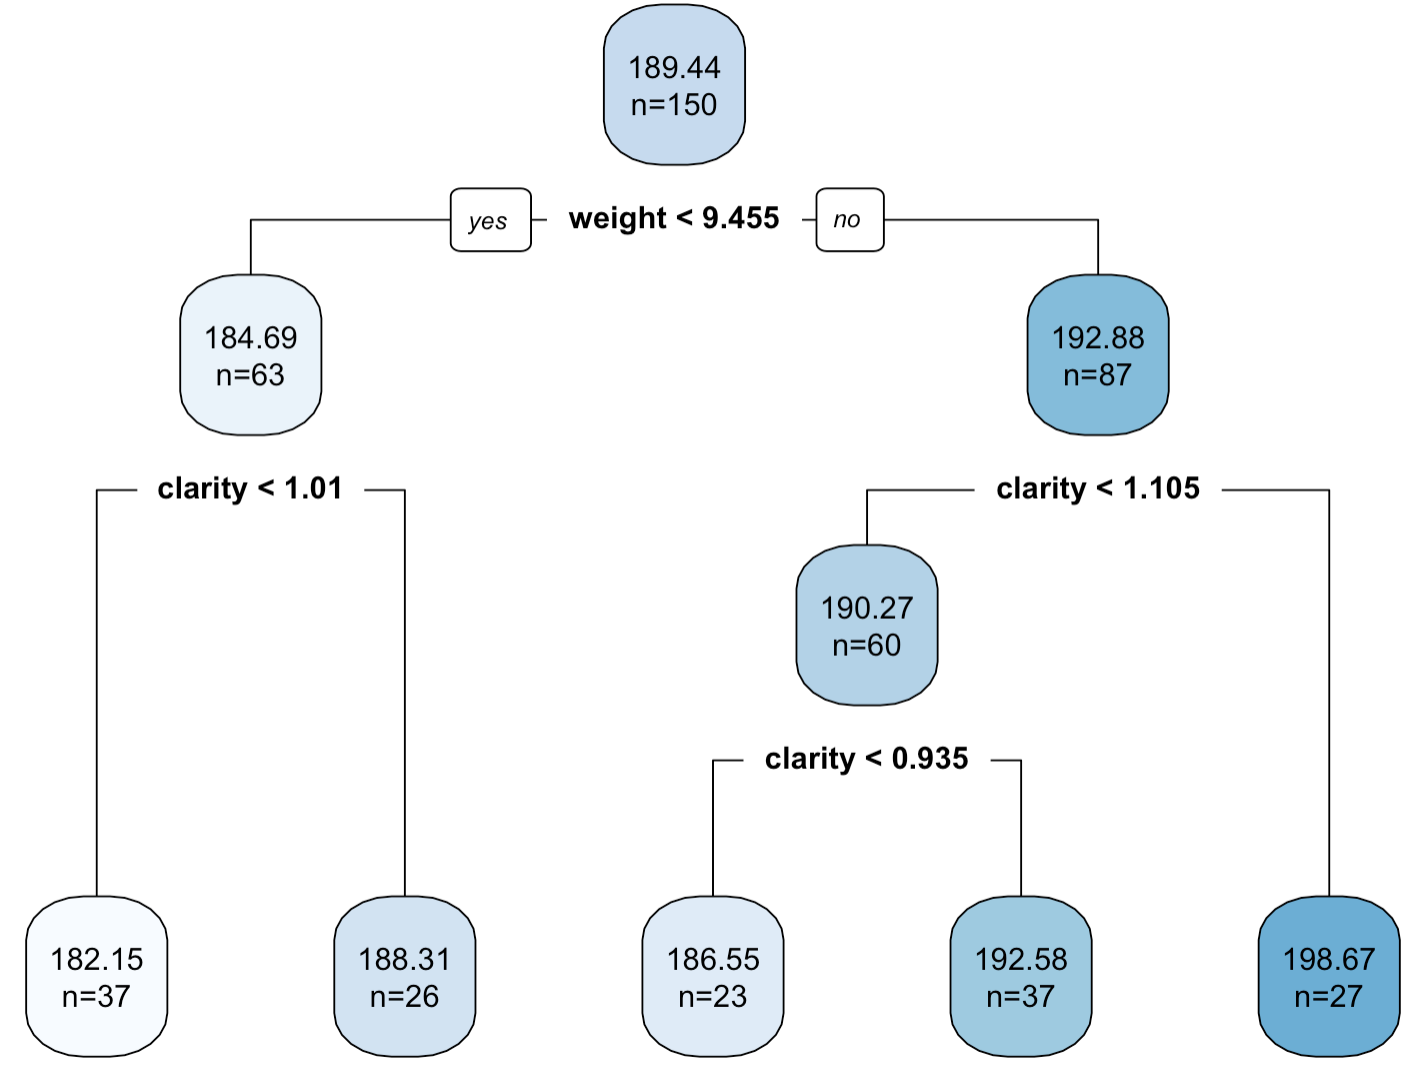
\includegraphics[scale=.55]{TreeDiamond.png}\\
The numbers provided at the terminal node,  denote the the corresponding predicted response ans the number of observations are allocated to the specific terminal node.  Answer the following questions based on the estimated tree given in this problem. 
}
}




\begin{enumerate}
\item  \ExamQuestion{  \TextInBoxOne{5.75in}{  Let $ \alpha(\text{T})$ denote the usual complexity measure obtained by the number of the terminal node of the tree or the number of decision regions that it corresponds.  {\bf What is the value of $\alpha(\text{T}^{*})$?}
}}{\vspace{.1in}
}{\hspace{-.2in}Total Score: 2}\\
\vspace{.5in}

\item  \ExamQuestion{  \TextInBoxOne{5.75in}{   Write down/describe the  different decision regions that the tree corresponds to.
}}{\vspace{.1in}
}{\hspace{-.2in}Total Score: 5}\\
\vspace{4.8in}

\item  \ExamQuestion{  \TextInBoxOne{5.75in}{  Based on the given output, what is the predicted response of a point that has the following values for the corresponding covariates\\
\vspace{-.35in}
\begin{center}
\begin{tabular}{|c|c|c|}
\hline
weight    & clarity & color  \\ \hline
12 & 1.0 & 4.0\\
\hline
\end{tabular}?
\end{center}
}}{\vspace{.1in}
}{\hspace{-.2in}Total Score: 3}\\
\vspace{2in}

\end{enumerate}







\TextInBoxTwo[lightBlueThree]{6.5in}{ \centering  \bf\HLT[white]{ \large Part-III}\\
  \begin{center}
 Answer the following descriptive type questions.  Show your steps to get  full credit. 
 \end{center}
 %You do not need any further justification to your answers. 
 }



\item \TextInBoxTwo[lightBlueTwo]{6.25in}{ 
 \TextInBoxOne{6.1in}{Let $\hat{\Sigma}$ be an estimated variance covariance matrix from a data set with 7 variables denoted as $X_1, \ldots , X_7$.  As the variance covariance matrix is non negative definite matrix, a spectral decomposition of the matrix is possible to be done.  Based on a computation procedure to applied to  $\hat{\Sigma}$, the following spectral decomposition is obtained:
$$\hat{\Sigma}:=\Gamma \Lambda \Gamma^T, \text{ where }$$
$$\Gamma=\RowVec{ \Col{-0.92,0,0.39,0,0,0,0}, \Col{0,0.98,0,0.05,0,0,-0.17}, \Col{0.39,0,0.92,0,0,0,0}, \Col{0,-0.04,0,-0.87,0,0,-0.49}, \Col{0,0,0,0,-0.73,0.68,0}, \Col{0,0,0,0,0.68,0.73,0}, \Col{0,-0.17,0,0.49,0,0,-0.85}
  }$$
$$\Lambda=\RowVec{ \Col{25,0,0,0,0,0, 0} , \Col{0,20,0,0,0,0,0} , \Col{0,0,2.4,0,0,0,0} , \Col{0,0,0,1.1,0,0,0} , \Col{0,0,0,0,1,0,0} , \Col{0,0,0,0,0,0.4,0} , \Col{0,0,0,0,0,0,0.1} }.$$
Note that $\Gamma$ is an Orthogonal-Matrix i.e. $\Gamma^T\Gamma=\Gamma\Gamma^T=\text{I}_{_{7\times 7}}$, the identity matrix of dimension $7\times 7$ while,  $\Lambda$ is a diagonal matrix with non-negative diagonal elements.  Also, note that the columns of the matrix $\Gamma$ comprises of the eigen-vectors of the matrix $\hat{\Sigma}$ while the diagonal elements of the matrix $\Lambda$ refers to the corresponding eigen-values of $\hat{\Sigma}$. Answer the following questions based on the results provided above.
}}

\begin{enumerate}
\item \ExamQuestion{ \TextInBoxOne{5.7in}{ What are the equations for the first {\bf  two principal components}, $\text{PC}_1$,  and $\text{PC}_2$ of the observed data? 
}}{ \\ \vspace{3in}
}{\hspace{-.2in}Total Score: 2+2}\\


\item \ExamQuestion{ \TextInBoxOne{5.7in}{What is the loading of $\text{PC}_{1}$ on the different variables?
}}{ \\
}{\hspace{-.2in}Total Score:  3}\\
\vspace{1in}



%
%\item \ExamQuestion{ \TextInBoxOne{5.7in}{Derive the co-variance between  $\text{PC}_{1}$ and $\text{PC}_{2}$.
%}}{ \\
%}{\hspace{-.2in}Total Score: 10 }\\


\item \ExamQuestion{ \TextInBoxOne{5.7in}{ Draw a scree plot of the importance factors for the principal components.  Based on the scree-plot,  identify the optimum number of components (say $m$) that would be adequate to capture the variability present in the observed data.  
}}{ \\
}{\hspace{-.2in}Total Score: 4+1 }\\

\includegraphics[scale=.4]{Grid_Scree.png}\\
\vspace{.1in}

\item \ExamQuestion{ \TextInBoxOne{5.7in}{What is the  percentage of total variability that is captured by the first $m$ principal components of the data.  {(\small Here $m$ is the optimum number of components that you have decided in the previous part of the problem. )}
}}{ \\
}{\hspace{-.2in}Total Score: 5 }\\	
\vspace{1in}

\item \ExamQuestion{ \TextInBoxOne{5.7in}{If a specific observed data point is:\\ 
$\Row{X_ 1 = 3.0,X_ 2 = 4.0,X_ 3 = 2.0,X_ 4 = 0,X_5=0 , 6 = 0, X_7 = 0}$\\
What is the score of the plot along the {\bf first } principal components?
}}{ \\
}{\hspace{-.2in}Total Score: 3 }\\	
\vspace{1in}


\item \ExamQuestion{ \TextInBoxOne{5.7in}{Derive the variance of $\text{PC}_{1}$.
}}{ \\
}{\hspace{-.2in}Total Score: 5 }\\
\vspace{4in}
\end{enumerate}










\item \TextInBoxTwo[lightBlueTwo]{6.25in}{ 
 \TextInBoxOne{6.1in}{
Consider a clustering problem of bivariate data with the following distance matrix: \\
\begin{center}
\begin{tabular}{|l|l|l|l|l|}
\hline
 & A   & B      & C   & D   \\ \hline
A & 0   & 7 & 4 & 6 \\ \hline
B & 7 & 0    & 4.5 & 3 \\ \hline
C & 4 & 4.5  & 0   & 1.5 \\ \hline
D & 6 & 3  & 1.5 & 0   \\ \hline
\end{tabular}
\end{center}
}}

\begin{enumerate}
\item \ExamQuestion{ \TextInBoxOne{5.7in}{ Complete the tables in the next page and construct a Dendogram for hierarchical agglomerative clustering  using the {\bf complete-linkage} procedure.
}}{\\ \Ans 
}{\hspace{-.2in}Total Score: 4+3}\\
{\Large
Step1: 
\begin{tabular}{|l||l|l|l|l|}
\hline
  \hspace{.9in} & A  \hspace{.7in} & B   \hspace{.7in}     & C \hspace{.7in}    & D  \hspace{.7in}   \\ \hline\hline
A & 0   & 7 & 4 & 6\\ \hline
B & 7 & 0    & 4.5 & 3 \\ \hline
C & 4 & 4.5  & 0   & 1.5 \\ \hline
D & 6 & 3  & 1.5 & 0   \\ \hline
\end{tabular}\\
\vspace{.1in}\\
Step2: 
\begin{tabular}{|l||l|l|l|}
\hline
\hspace{.9in} & \hspace{1in}   & \hspace{1in}      &  \hspace{1in}     \\ \hline\hline
&   &   &    \\ \hline
 &  &     &    \\ \hline
&  &   &     \\ \hline
& &   &  \\ \hline
\end{tabular}

\vspace{.1in}
Step3: 
\begin{tabular}{|l||l|l|}
\hline
\hspace{.9in} & \hspace{1in}   & \hspace{1in}           \\ \hline\hline
&   &      \\ \hline
 &  &       \\ \hline
&  &     \\ \hline
\end{tabular}

}
\begin{center}

\includegraphics[scale=.4]{DendoPlot.png}\\
\end{center}
\vspace{.01in}

\item \ExamQuestion{ \TextInBoxOne{5.7in}{ Based on the Dendogram that you have obtained, identify the clustering assignments of the points if there is only two clusters in the data. 
}}{ \\ \vspace{3in}
}{\hspace{-.2in}Total Score: 3}\\
\end{enumerate}







\item \TextInBoxTwo[lightBlueTwo]{6.25in}{ 
 \TextInBoxOne{6.1in}{
Consider a clustering problem of bivariate data:
$A=\ColVec{6,2},
B=\ColVec{7,3},
C=\ColVec{3,2},
D=\ColVec{5,4},
E=\ColVec{1,1} $
%F=\ColVec{4,0},
where the points are labeled as A, B, C, D, E, F. The Euclidean distance between the points are provided in the distance matrix below:
\begin{center}
\vspace{-.1in}
\begin{tabular}{|l||l|l|l|l|l|l|}
\hline
  & A    & B    & C    & D    & E       \\ \hline\hline
A & 0     & 1.41 & 3 & 2.24  & 5.10         \\ \hline
B & 1.41 & 0    & 4.12    & 2.24 & 6.32  \\ \hline
C & 3     & 4.12    & 0    & 2.83  & 2.24  \\ \hline
D & 2.24 & 2.24 & 2.83  & 0    & 5    \\ \hline
E & 5.10    & 6.32 & 2.24 & 5 & 0        \\ \hline
\end{tabular}
\vspace{-.2in}
\end{center}
\vspace{.2in}
 During an iteration of the K-means algorithm with 2 clusters, the points $\{A,B,D\}$ are assigned to Cluster1 and the rest of the points namely $\{C,E\}$ to the Cluster2. 
}}

\begin{enumerate}
\item \ExamQuestion{ \TextInBoxOne{5.7in}{  Identify the resulting cluster centers for both the groups at the beginning   of the next iteration.
}}{ \\ \vspace{2.5in}
}{\hspace{-.2in}Total Score: 5}\\

\item \ExamQuestion{ \TextInBoxOne{5.7in}{ Compute the Withing Group Sum of Squares for  clusters provided in part(a).  
}}{ \\ \vspace{3in}
}{\hspace{-.2in}Total Score: 5}\\
\end{enumerate}








\item \TextInBoxTwo[lightBlueTwo]{6.25in}{ 
 \TextInBoxOne{6.1in}{Consider the following diagram of a Perceptron:\\
\begin{center}
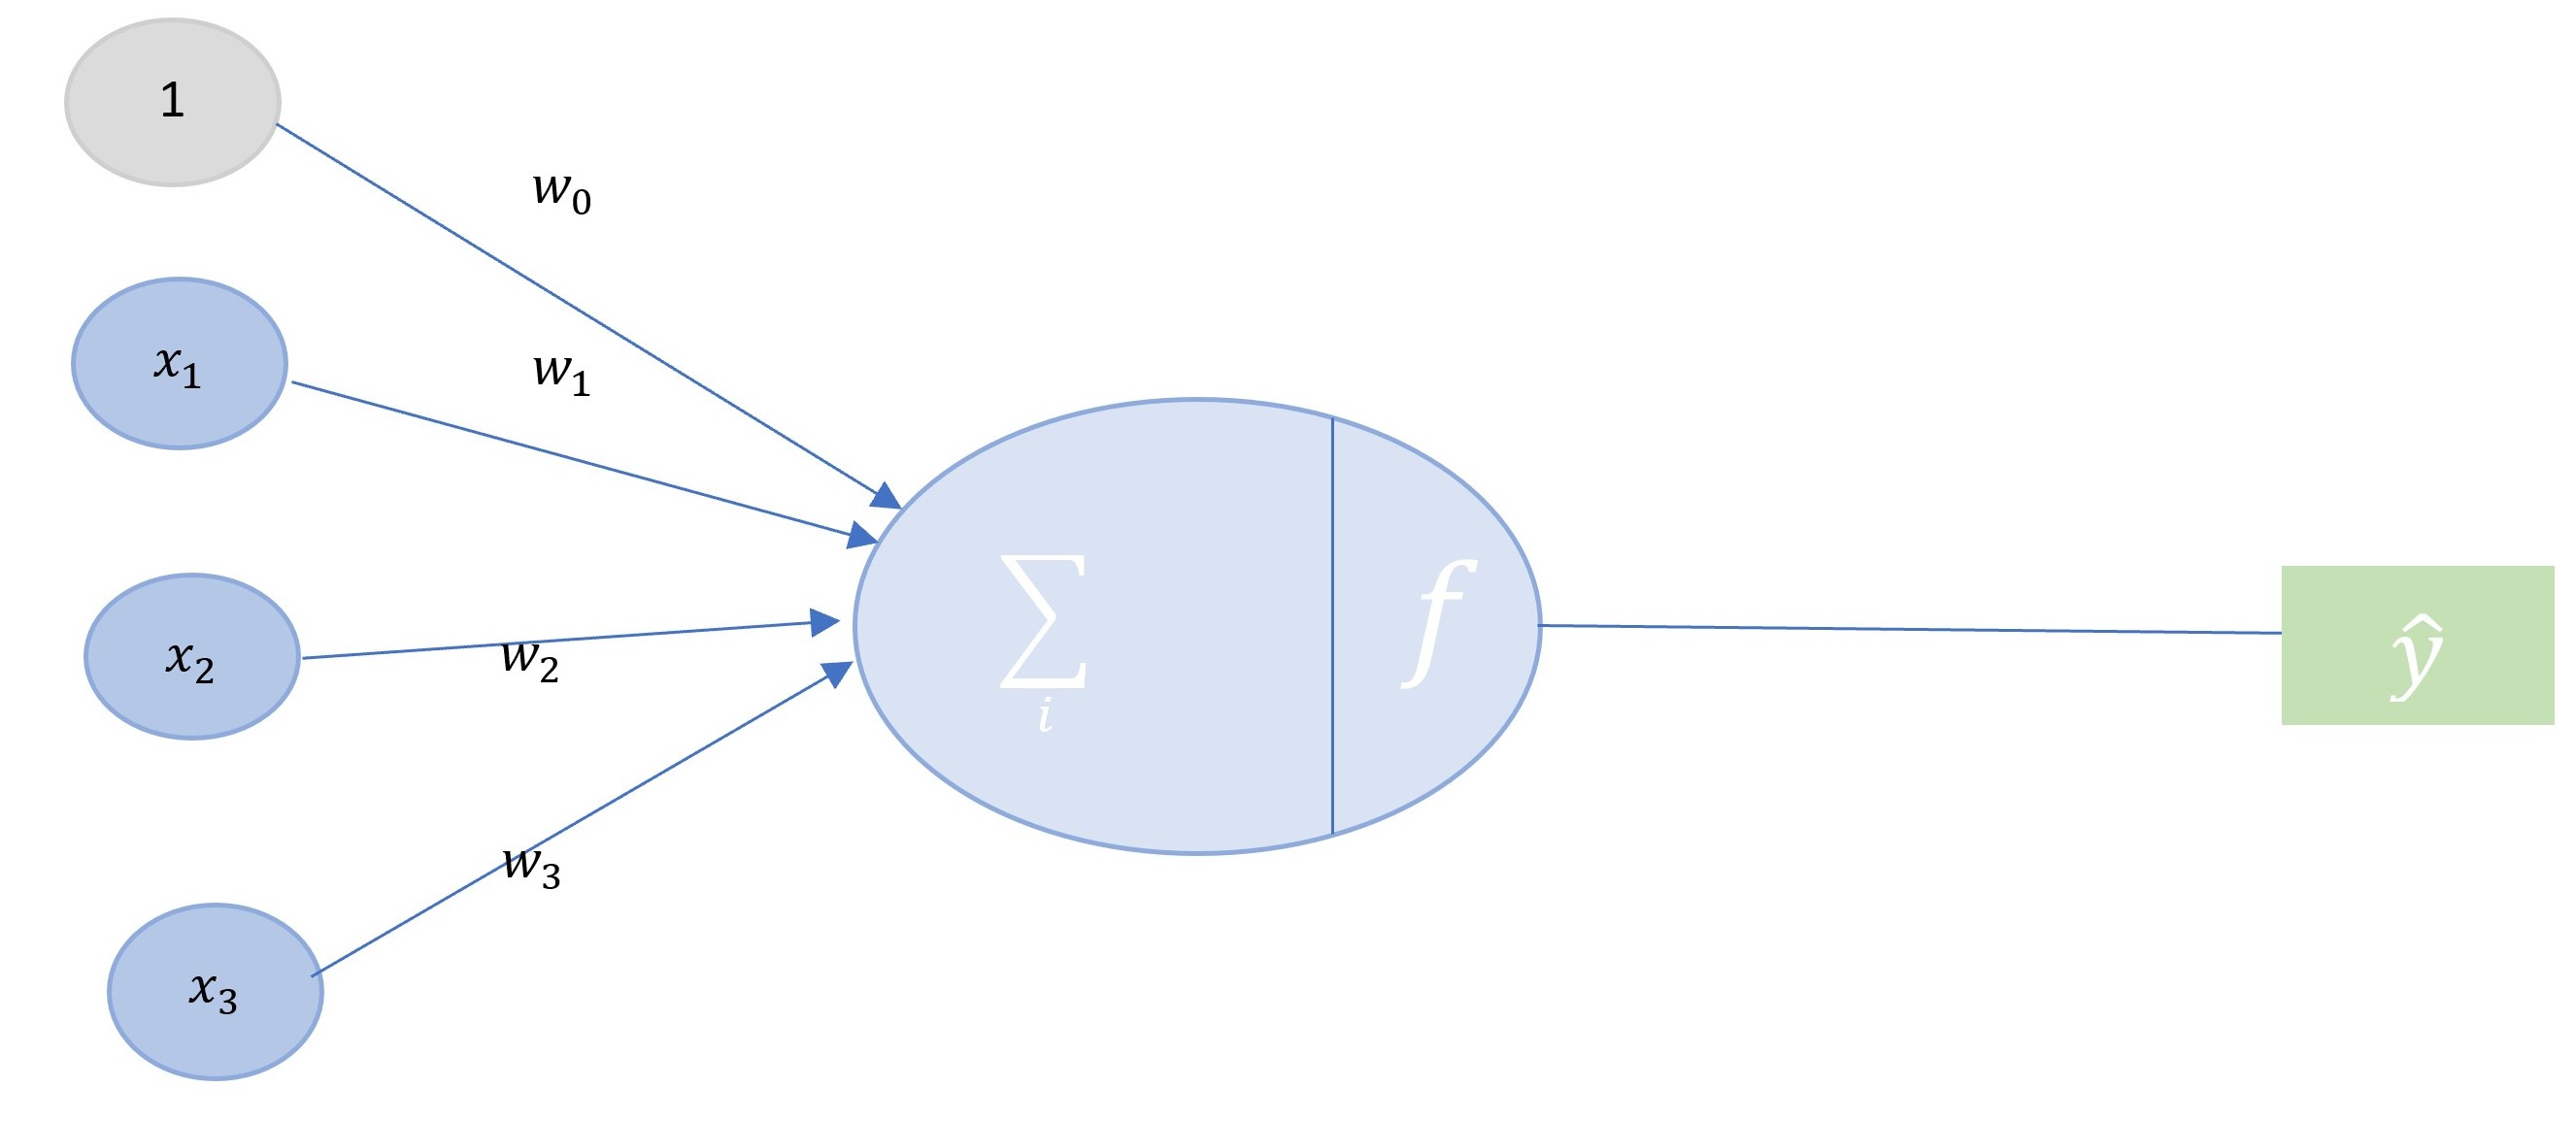
\includegraphics[scale=.3]{Perceptron_img.jpg}
\end{center}
Let the weights are given to be $\w_0=5$, $\w_1=2$, $\w_2=-3$, $\w_3=1$.  
}}

\begin{enumerate}
\item \ExamQuestion{ \TextInBoxOne{5.7in}{Write down the mathemetical formulation of the above Perceptron.  Keep the nonlinear function to be the generic $f$ in your expression.
}}{ \\ \vspace{2in}
}{\hspace{-.2in}Total Score: 3}\\

%\item \ExamQuestion{ \TextInBoxOne{5.7in}{If we consider the nonlinear function $f$ to be the Sigmoid function, then what would be the output from the above Perceptron?Assume, the observed covariates/imputs are given as
%$x_1=4, x_2=1, X_3=-1$.  
%}}{ \\ \vspace{3in}
%}{\hspace{-.2in}Total Score: 5}\\

\item \ExamQuestion{ \TextInBoxOne{5.7in}{ If we consider the nonlinear function $f$ to be the {\bf ``ReLU''} (Rectified Linear Unit) function, then what would be the output from the above Perceptron? Assume, the observed covariates/imputs are given as
$x_1=0, x_2=1, x_3=0$.  Note that ReLU$(x)=$Max$(x,0)$.
}}{ \\ \vspace{1in}
}{\hspace{-.2in}Total Score: 2}\\
%\item \ExamQuestion{ \TextInBoxOne{5.7in}{Write down the mathemetical formulation of the above Perceptron.  Keep the nonlinear function to be the generic $f$ in your expression.
%}}{ \\ \vspace{3in}
%}{\hspace{-.2in}Total Score: 5}\\
\vspace{1.4in}
\end{enumerate}


%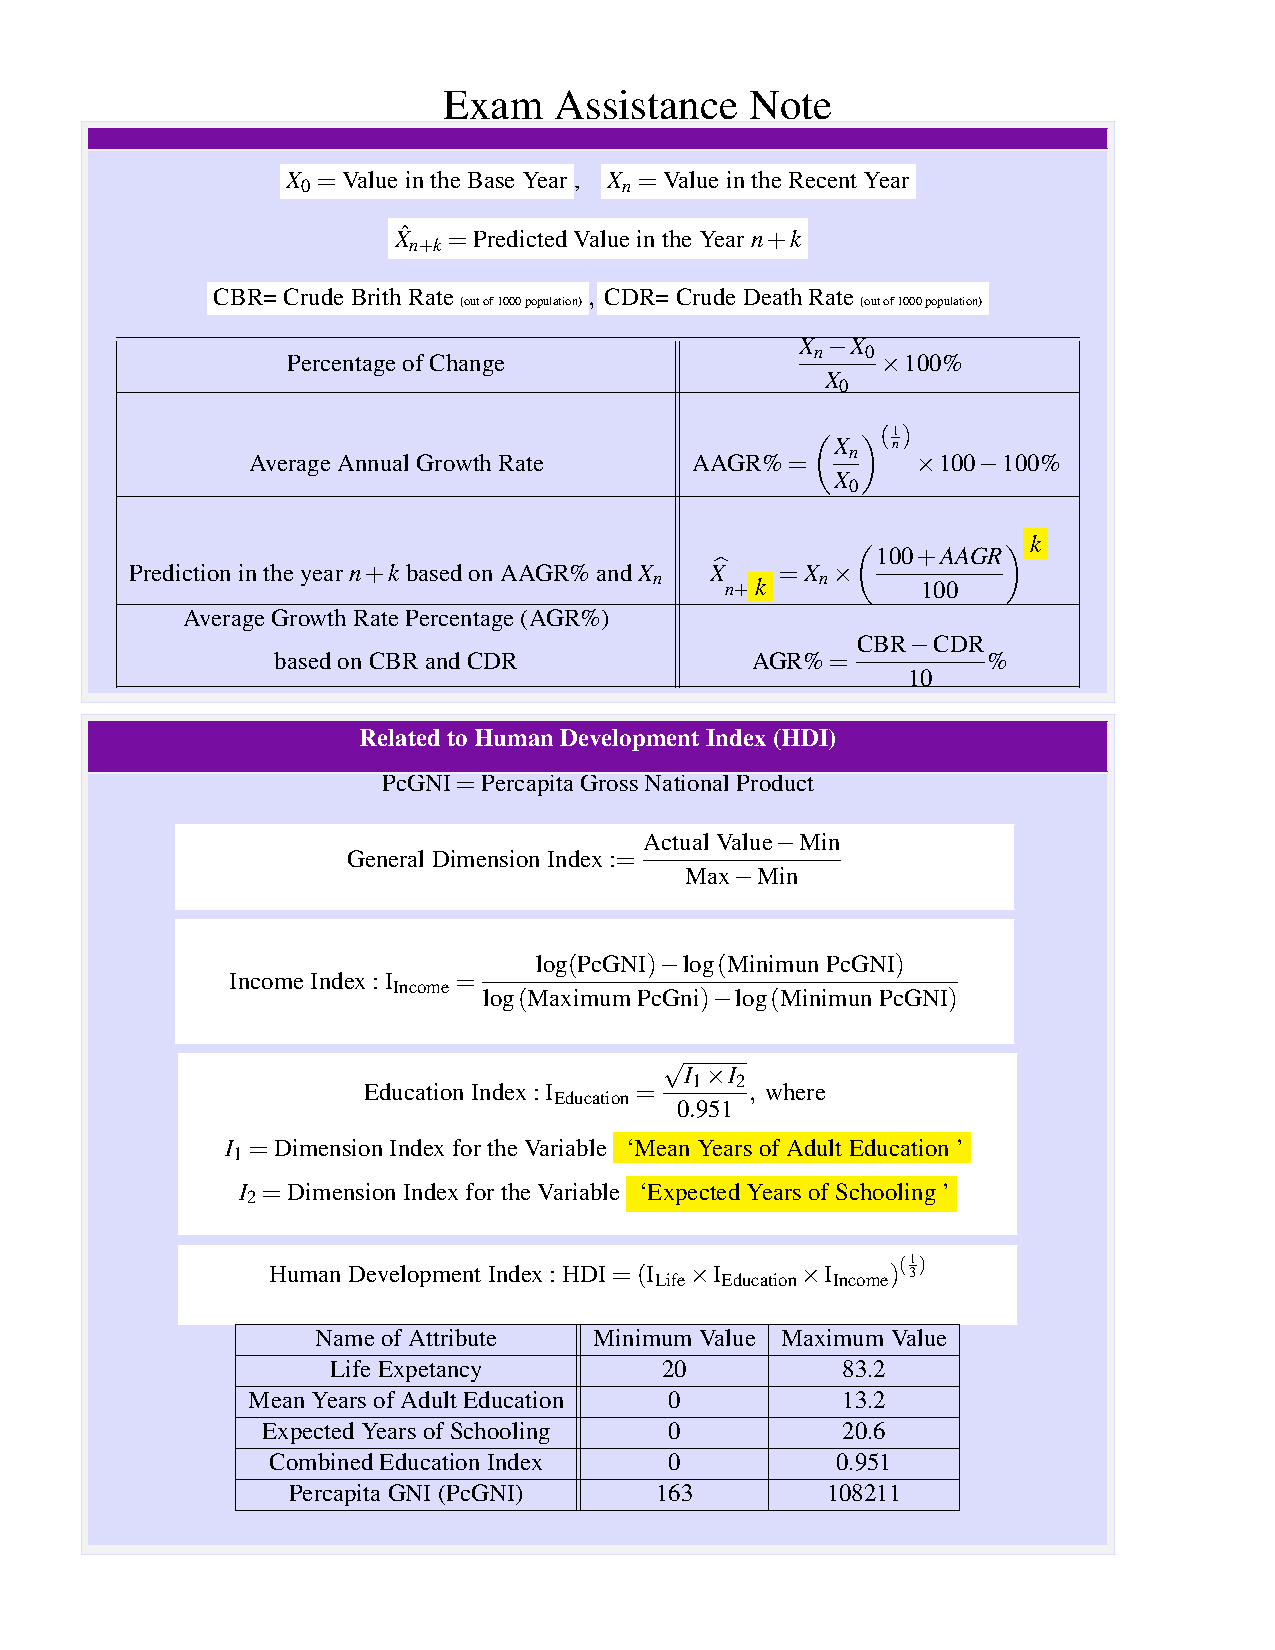
\includepdf[pages=-]{ExamAssistanceNote_STAt101.pdf}





\end{enumerate}


\hrule
\hrule
\TextInBoxTwo[gray!25]{6.65in}{
\begin{center}
\small !!! All the Best !!! 
\end{center}
}
\hrule
\hrule
\end{document}